\section{Durchführung und Aufbau}
\label{sec:Durchführung}
Die Verschaltung des Versuches ist in Abbildung \ref{fig:Aufbau} zu sehen. Die durch die Townsend-Lawine verusachte Ladungen auf der Mantelfläche fließt über einen Widerstand ab und erzeugen einen Spannungsimpuls, welcher über den Kondensator ausgekoppelt wird. Anschließend wird nach Verstärkung der Impulse im Zähler die Impulsrate angezeigt oder im Oszilloskop visualisiert.
\begin{figure}
  \centering
  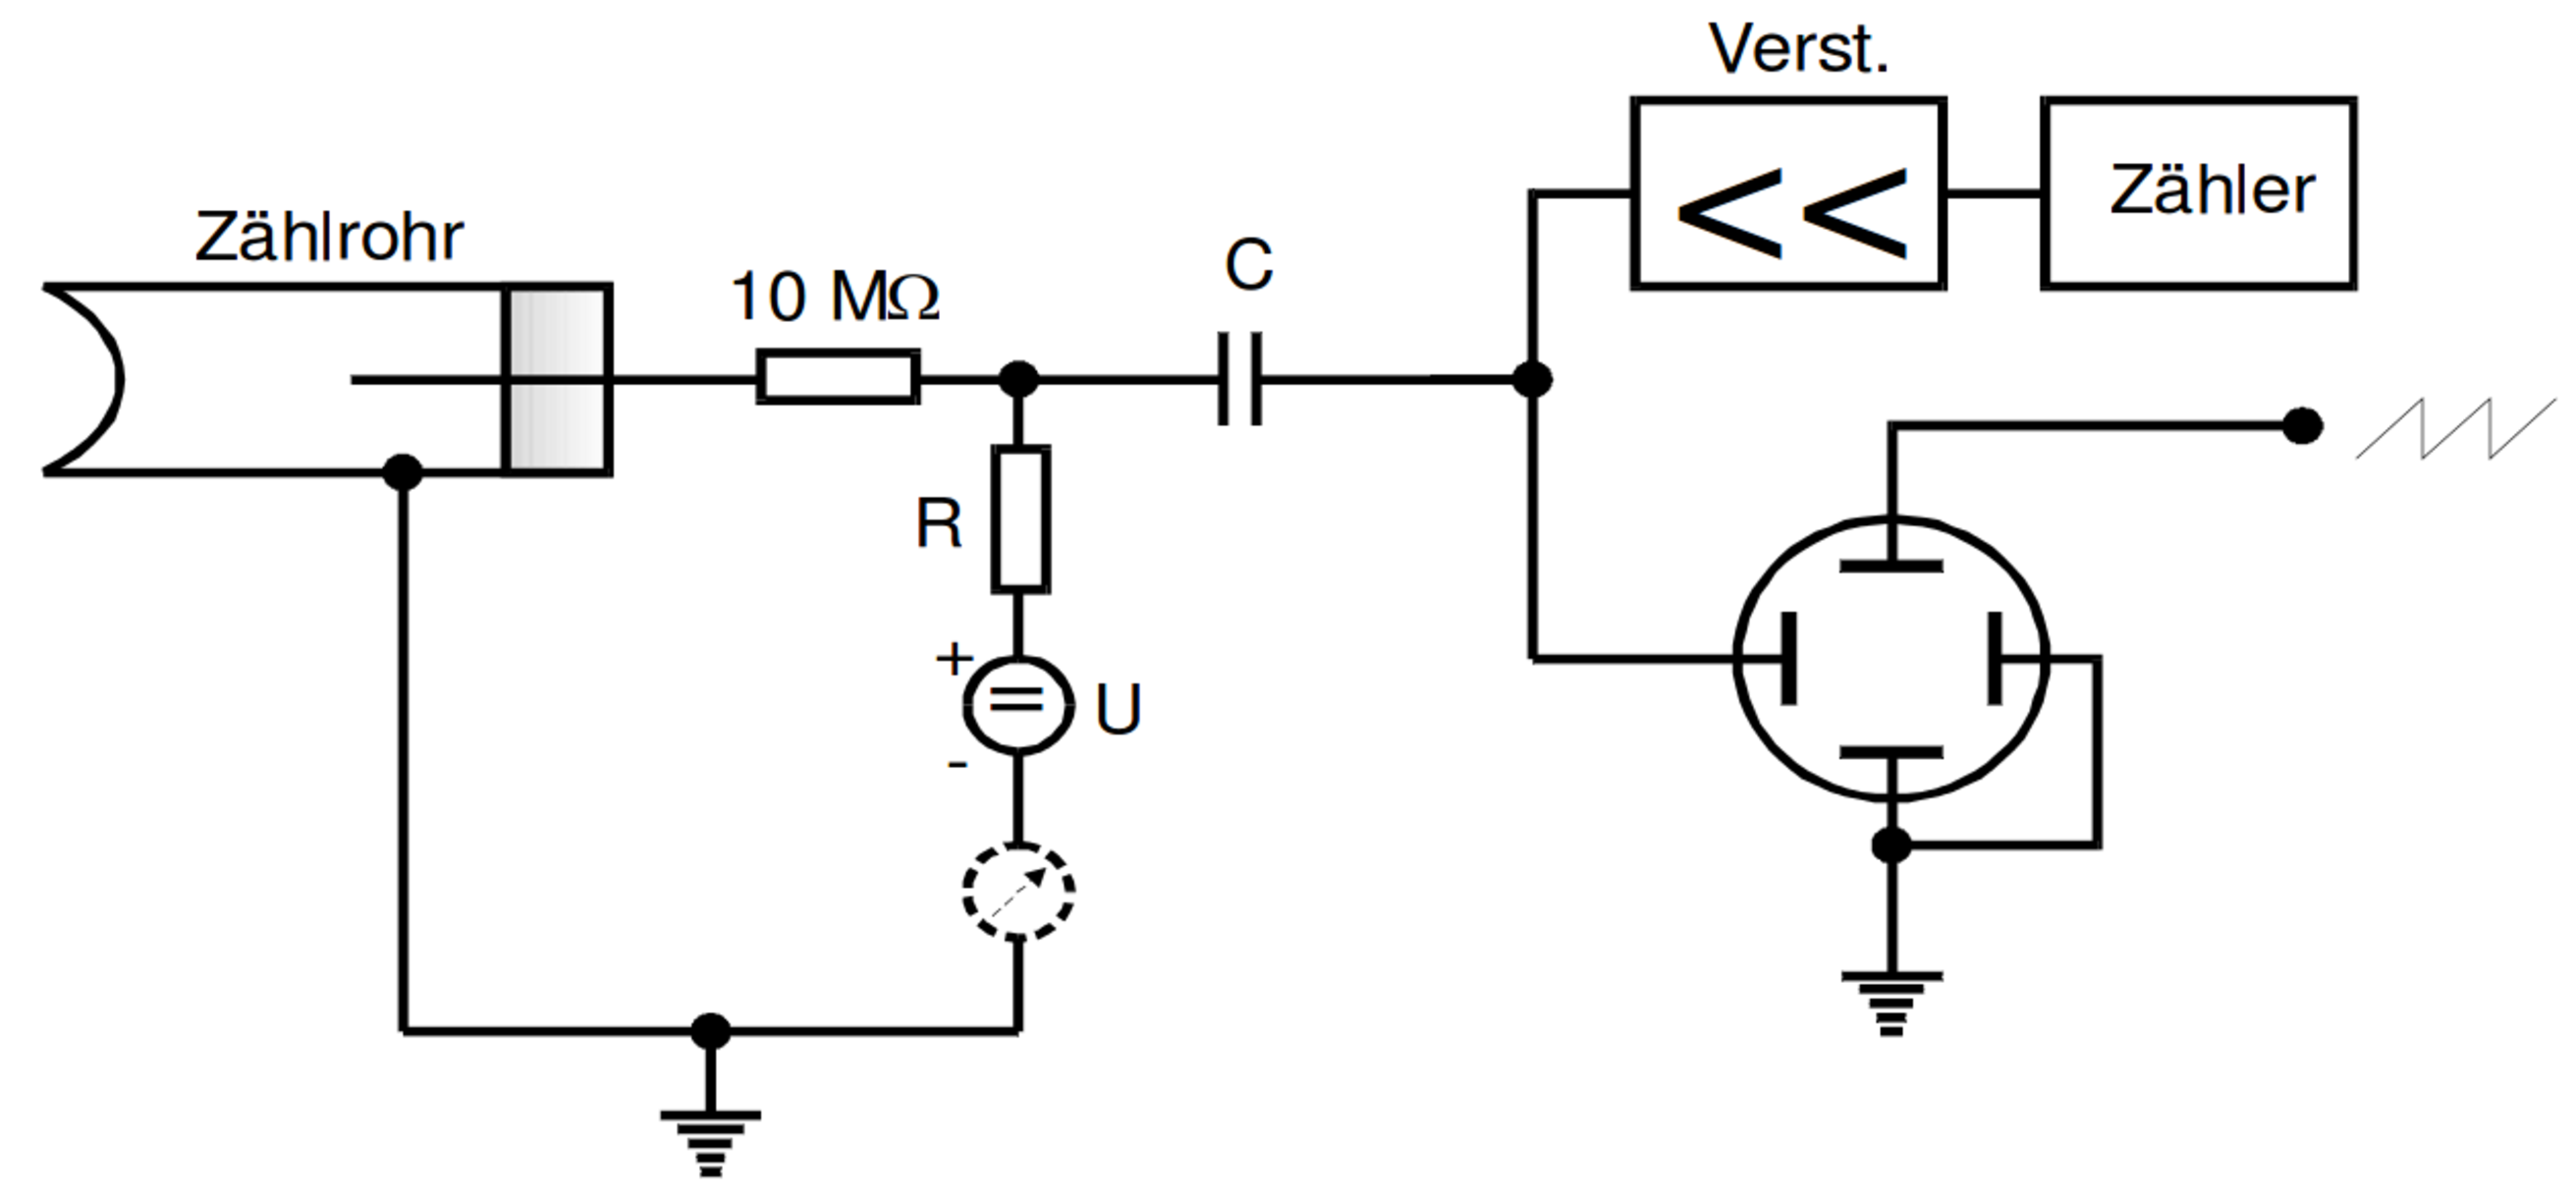
\includegraphics[height=4cm]{picture/Aufbau.pdf}
  \caption{Modell des Versuchsaufbau \cite{sample}}
  \label{fig:Aufbau}
\end{figure}
\subsection{Messprogramm}
Zunächst wird vor das Zählrohr im geeigneten Abstand ein Thallium 204 Präperat gestellt. Anschließend wird sowohl der Strom, als auch die Impulsrate in Abhängigkeit der Betriebsspannung gemessen. Es werden 20 Messwerte genommen die an den Randstellen des Plateaus dichter gewählt werden.
Aus dem Oszilloskopbild wird die Totzeit sowie die Nachentladung gemessen. Dabei muss eine geeignete Intensität durch Positionierung des Präperats gewährleistet werden. Für die Nachentladung wird sowohl einmal für eine Betriebsspannung von 350\,V als auch von 700\,V der Abstand zwischen Primär- und Nachentladungsimpuls auf dem Oszilloskop vermessen.

Zuletzt wird die Totzeit anhand der Zwei-Quellen-Methode bestimmt. Dabei wird zuerst die Zählrate des ersten Präperats bestimmt und anschließend ein weiteres Präperat auf das Geiger-Müller-Zählrohr gerichtet und die Impulsrate bestimmt. Das erste Präperat wird nun aus dem Strahlengang genommen und die Impulsrate des zweiten Präperats bestimmt.
